%%%%%%%%%%%%%%%%%%%%%%%
%%% DOCUMENT SETTINGS
%%%%%%%%%%%%%%%%%%%%%%%
\documentclass[11pt]{exam}
\printanswers % Uncomment to show answers
%%%%%%%%%%%%%%
%%% PACKAGES
%%%%%%%%%%%%%%
\usepackage{amsmath,amsfonts,amssymb,amsthm}
\usepackage{bbm}
\usepackage{enumitem}
\usepackage{textcomp}
\usepackage[top = 2cm, bottom = 2cm, right = 1.2cm, left = 1.2cm, paper = a4paper, headheight = 6cm]{geometry}
\usepackage{xcolor}
\usepackage{graphicx}
%----------------------------------- Tikz
\usepackage{tikz}
\usepackage{pgfplots}
\pgfplotsset{compat=1.17}
\usepgfplotslibrary{fillbetween}
\usetikzlibrary{shapes,arrows,matrix,positioning,calc}
\newcommand{\tikzmark}[1]{\tikz[baseline,remember picture] \coordinate (#1) {};}
%%%%%%%%%%%%%%%%%%%%%%%%%%
%%% Colors
%%%%%%%%%%%%%%%%%%%%%%%%%%
\definecolor{firebrick3}{RGB}{207, 33, 32}
\definecolor{deepskyblue3}{RGB}{0, 155, 206}
\definecolor{darkolivegreen3}{RGB}{163, 207, 91}
%%%%%%%%%%%%%%%%%%%%%%%%%%
%%% MACROS AND COMMANDS
%%%%%%%%%%%%%%%%%%%%%%%%%%
\newcommand{\N}{\mathbb{N}}
\newcommand{\R}{\mathbb{R}}
\makeatletter
\renewcommand{\@makefnmark}{\textsuperscript{\arabic{footnote}}}
\renewcommand{\thefootnote}{\arabic{footnote}}
\makeatother
\setcounter{footnote}{0}
\newcommand{\BAR}{%
    \hspace{-\arraycolsep}%
    \strut\vrule
    \hspace{-\arraycolsep}%
}
%%%%%%%%%%%%%%%%%%%%%%%%%%%%%%%%%
%%% HEADER AND FOOT
%%%%%%%%%%%%%%%%%%%%%%%%%%%%%%%%%
\newcommand{\degree}{Bachelor in Philosophy, Politics and Economics}
\newcommand{\shortdeg}{PPE}
\newcommand{\exam}{Final Exam -- Retake}
\newcommand{\subject}{Mathematics}
\newcommand{\theyear}{2025/26}
\newcommand{\ccauthor}{A. G. Azze}
\newcommand{\thedate}{Jan 30, 2026}
\newcommand{\university}{CUNEF Universidad}
\pagestyle{headandfoot}
\header{\degree \\ \subject\ - \theyear}{}{\thedate \\ \ccauthor}
\footer{\university}{}{\thepage}

%%%%%%%%%%%%%%%%%%%%%%%%%
%%% DOCUMENT CONTENT
%%%%%%%%%%%%%%%%%%%%%%%%%
\begin{document}

%--- Instructions ---%
\begin{center}

    {\Huge \textbf{\exam{}}}

    \begin{flushright}
        \vspace{-0cm}
        \textbf{Time Limit:} 120 minutes
    \end{flushright}
    \vspace{-0.15cm}

    \fbox{\parbox{\textwidth}{\centering
        \begin{enumerate}[leftmargin = 0.5cm, label = $\bullet$, rightmargin = 0.2cm]
            \item \textbf{Every non-trivial calculation and claim in the exam must be properly justified.}
            \item The use of calculators is not necessary and therefore not allowed.
            \item Digital devices such as mobile phones, tablets, and laptops, as well as internet access, are forbidden.
        \end{enumerate}
    }}
\end{center}
%--- Instructions ---%

\begin{questions}

%%%%%%%%%%%%%%%%%%%%%%%%%%%%%%%%%%%%%%%%%%%%%%%%%%%%%%%%%%%%
% Question 1
%%%%%%%%%%%%%%%%%%%%%%%%%%%%%%%%%%%%%%%%%%%%%%%%%%%%%%%%%%%%
\question[2]
A market for self-driving cars is described by the inverse supply and demand functions
\[
p_S(q)=2^{q-2},
\qquad
p_D(q)=\frac{12}{1 + \sqrt{q}},
\qquad q\ge 0.
\]

\begin{minipage}{0.6\textwidth}
\begin{enumerate}[leftmargin = 0.5cm, label = (\alph*), rightmargin = 0.2cm]
    \item Prove that the market has an equilibrium at $p^* = 4$. Find $q^*$.
    \item Provided that the Consumer Surplus (area $CS$ in Figure 1) equals $CS\approx 5.63$,
    compute the Total Consumer Value
    \[
        TCV = \int_0^{q^*} p_D(q)\, dq.
    \]
    \item Compute the Producer Surplus (area $PS$ in Figure 1). \\
    {\footnotesize Hint: $f'(x) = 2^x$ for $f(x) =\frac{2^x}{\ln 2}$.}
    \item Use the tangent line of $p_D$ at $q=4$ to estimate $p_D(3.9)$.
\end{enumerate}
\end{minipage}
\hspace{0.5cm}
\begin{minipage}{0.34\textwidth}
\vspace{-0.5cm}
\begin{center}
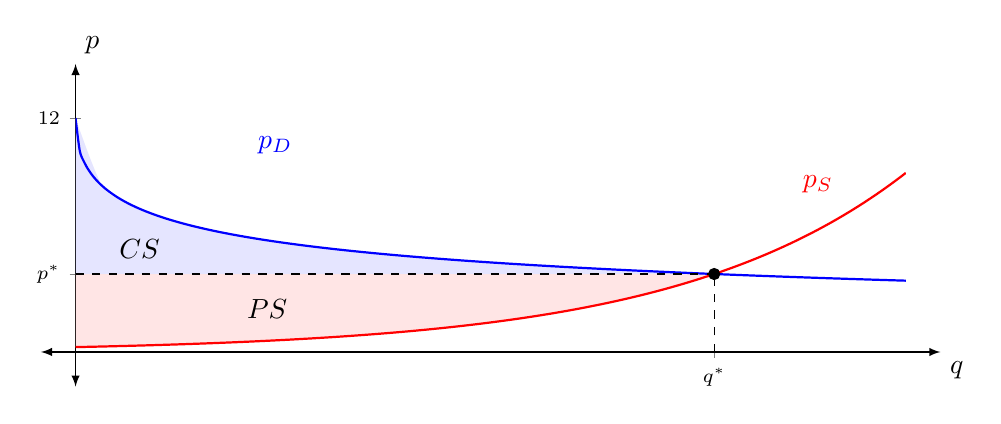
\begin{tikzpicture}
\begin{axis}[
    width=\textwidth,
    height=4.8cm,
    axis lines=middle,
    xmin=0, xmax=5.2,
    ymin=0, ymax=13,
    ytick={0,4,12},
    xtick={0,4},
    xticklabels={$0$, $q^*$},
    yticklabels={$0$, $p^*$, $12$},
    scaled ticks=false,
    ticklabel style={font=\scriptsize},
    xlabel=$q$, ylabel=$p$,
    axis line style={latex-latex, shorten >=-12.5pt, shorten <=-12.5pt},
    xlabel style={at={(ticklabel* cs:1)}, xshift=12.5pt, anchor=north west},
    ylabel style={at={(ticklabel* cs:1)}, yshift=12.5pt, anchor=south west},
]

% Shaded areas (requires \usepgfplotslibrary{fillbetween} in the preamble)
\path[name path=demand_left] plot[smooth, domain=0:4] (\x, {12/(1+sqrt(\x))});
\path[name path=supply_left] plot[smooth, domain=0:4] (\x, {2^(\x-2)});
\path[name path=price] (axis cs:0,4) -- (axis cs:4,4);

\addplot[fill=blue!20, opacity=0.5] fill between[of=demand_left and price];
\addplot[fill=red!20,  opacity=0.5] fill between[of=price and supply_left];

% Curves
\addplot[thick, red, samples=201, smooth, domain=0:5.2] {2^(x-2)};
\addplot[thick, blue, samples=201, smooth, domain=0:5.2] {12/(1 + sqrt(x))};

% Equilibrium point + guides
\addplot[mark=*] coordinates {(4,4)};
\addplot[dashed] coordinates {(4,0) (4,4)};
\addplot[dashed] coordinates {(0,4) (4,4)};

% Labels
\node at (axis cs:4.65,8.6) {$\textcolor{red}{p_S}$};
\node at (axis cs:1.25,10.6) {$\textcolor{blue}{p_D}$};
\node at (axis cs:0.4,5.3) {$CS$};
\node at (axis cs:1.2,2.2) {$PS$};

\end{axis}
\end{tikzpicture}

{\small Figure 1}
\end{center}
\end{minipage}

% Solution
\begin{solution}[0cm]
\begin{enumerate}[leftmargin = 0.5cm, label = (\alph*), rightmargin = 0.2cm]

\item
At equilibrium, $p_S(q^*)=p_D(q^*)=p^*$.  
Since $p^*=4$, from $2^{q^*-2}=4=2^2$ we get $q^*-2=2$, hence $q^*=4$.  
Then $p_D(4)=\dfrac{12}{1+\sqrt4}=\dfrac{12}{3}=4$, so this is an equilibrium.

\item
$
TCV = CS + p^*q^* \approx 5.63 + 4\cdot 4 = 21.63.
$

\item Using the hint,
\[
PS=\int_0^{4}\left(4-2^{q-2}\right)dq
=16-\left[\frac{2^{q-2}}{\ln 2}\right]_{0}^{4}
=16-\frac{15}{4\ln 2}.
\]

\item
\[
p_D'(q)= -\frac{6}{\sqrt{q}\,(1+\sqrt{q})^2}
\quad\Rightarrow\quad
p_D'(4)=-\frac{1}{3}.
\]
Thus the tangent line at $q=4$ is
\[
L(q)=p_D(4)+p_D'(4)(q-4)=4-\frac{1}{3}(q-4),
\]
so
\[
p_D(3.9)\approx L(3.9)=4-\frac{1}{3}(-0.1)=4.033\ldots
\]

\end{enumerate}
\end{solution}


%%%%%%%%%%%%%%%%%%%%%%%%%%%%%%%%%%%%%%%%%%%%%%%%%%%%%%%%%%%%
% Question 2
%%%%%%%%%%%%%%%%%%%%%%%%%%%%%%%%%%%%%%%%%%%%%%%%%%%%%%%%%%%%
\question[3]
A company operates a small energy hub with three daily decision variables:
\begin{align*}
    x&=\text{MWh sent to Data Centers}, \\
    y&=\text{MWh sent to Battery charging},\\
    z&=\text{MWh reserved for Software services}.
\end{align*}

The hub has a fixed daily energy budget of \(120\) MWh.

Each MWh sent to Data Centers generates \(\$6\) of revenue, each MWh sent to Battery charging generates \(\$2\) of revenue, and each MWh reserved for Software services generates \(\$1\) of revenue. The normal-day revenue target is \(\$360\).

On \emph{stress-test days}, only a half of the Data Center allocation and a half of the Battery allocation can be delivered, while Software services still run fully. The stress-test revenue target is \(\$200\).

\begin{enumerate}[leftmargin=0.5cm,label=(\alph*)]
  \item Write the system of equations that determines \((x,y,z)\).
  \item Write the system in matrix form \(A\mathbf w=\mathbf b\), identifying \(A\), \(\mathbf w\), and \(\mathbf b\).
  \item Solve the system.
  \item Would there be a solution if the allocation remains the same on stress-test days?
\end{enumerate}

\begin{solution}[0cm]
\begin{enumerate}[leftmargin=0.5cm,label=(\alph*)]

\item Budget, normal-day revenue target, and stress-test revenue target:
\[
\begin{cases}
x+y+z=120,\\
6x+2y+z=360,\\
6\left(\frac{x}{2}\right)+2\left(\frac{y}{2}\right)+z=200,
\end{cases}
\qquad\text{i.e.}\qquad
\begin{cases}
x+y+z=120,\\
6x+2y+z=360,\\
3x+y+z=200.
\end{cases}
\]

\item With \(\mathbf w=(x,y,z)'\),
\[
A=
\begin{pmatrix}
1&1&1\\
6&2&1\\
3&1&1
\end{pmatrix},
\qquad
\mathbf b=
\begin{pmatrix}
120\\360\\200
\end{pmatrix}.
\]

\item Subtract the first equation from the second: \(5x+y=240\).
Subtract the first from the third: \(2x=80\), so \(x=40\).
Then \(y=240-5(40)=40\) and \(z=120-x-y=40\). Hence
\[
(x,y,z)=(40,\,40,\,40).
\]

\item If the allocation remains the same on stress-test days, the third equation would be
\(6x+2y+z=200\), which contradicts \(6x+2y+z=360\). Therefore the system would have \textbf{no solution}.

\end{enumerate}
\end{solution}

%%%%%%%%%%%%%%%%%%%%%%%%%%%%%%%%%%%%%%%%%%%%%%%%%%%%%%%%%%%%
% Question 3
%%%%%%%%%%%%%%%%%%%%%%%%%%%%%%%%%%%%%%%%%%%%%%%%%%%%%%%%%%%%
\question[2]
You are developing a large language model that you may release at any time $t\ge 0$ (years).
Its \emph{launch value} after $t$ years is
\[
V(t)=120(1+t).
\]
Because of competition and discounting, one dollar received at time $t$ is worth $e^{-t/2}$ dollars today.

\begin{enumerate}[leftmargin = 0.5cm, label = (\alph*), rightmargin = 0.2cm]
    \item Write the present-value function $P(t)$ of releasing at time $t$.
    \item Compute $\lim_{t\to\infty} P(t)$ and interpret it.
    \item Find the release time $t^*$ that maximizes $P(t)$, and the maximum present value.
    \item Suppose you must release by a deadline $T$. What would be the optimal release time if $T=0.6$? What if $T=3$? Explain.
\end{enumerate}

\begin{solution}[0cm]
\begin{enumerate}[leftmargin = 0.5cm, label = (\alph*), rightmargin = 0.2cm]

\item
$P(t)=V(t)e^{-t/2}=120(1+t)e^{-t/2}$.

\item
$\lim_{t\to\infty} 120(1+t)e^{-t/2}=0$, since the exponential decay dominates linear growth. Interpretation: waiting forever makes the present value vanish.

\item
Differentiating:
\[
P'(t)=120\left(e^{-t/2}-(1+t)\tfrac12 e^{-t/2}\right)
=120e^{-t/2}\left(1-\tfrac12-\tfrac12 t\right)
=60e^{-t/2}(1-t).
\]
Thus $P'(t)=0$ at $t=1$, with $P'(t)>0$ for $t<1$ and $P'(t)<0$ for $t>1$. Hence the (global) maximizer and its associated maximum are
\[
t^*=1,
\qquad
P(1)=120\cdot 2\cdot e^{-1/2}=240e^{-1/2}.
\]

\item
\begin{itemize}
\item If $T=0.6<1$, then $P$ is increasing on $[0, 0.6]$, so the constrained optimum is at $t^*=T=0.6$.
\item If $T=3>1$, then the unconstrained maximizer $t=1$ is feasible, so the optimum remains $t^*=1$.
\end{itemize}

\end{enumerate}
\end{solution}

%%%%%%%%%%%%%%%%%%%%%%%%%%%%%%%%%%%%%%%%%%%%%%%%%%%%%%%%%%%%
% Question 4
%%%%%%%%%%%%%%%%%%%%%%%%%%%%%%%%%%%%%%%%%%%%%%%%%%%%%%%%%%%%
\question[3]
A firm sells a subscription to an AI assistant. The \emph{present value} up to time $T$ is
\[
V(T)=\int_{0}^{T} U(t)\,e^{-t}\,dt,
\]
where the (time-dependent) utility flow is
\[
U(t)=
\begin{cases}
6t^2+2, & 0\le t\le 1,\\[4pt]
8e^{(t - 1)/2}, & t>1.
\end{cases}
\]

\begin{enumerate}[leftmargin = 0.5cm, label = (\alph*), rightmargin = 0.2cm]
    \item What is the domain of $U$?
    \item Is $U$ continuous on its domain? Justify.
    \item Compute $V(1)$. \\
    {\footnotesize Hint: $f'(x) = x^2 e^{-x}$ for $f(x) = -e^{-x}(x^2+2x+2)$.}
    \item Compute the perpetual value $\int_{0}^{\infty} U(t)e^{-t}dt$.
    \item If instead $U(t)=2/(1+t^2)$, provide an upper bound for $\int_{0}^{\infty}U(t)e^{-t}dt$.
\end{enumerate}

% Solution
\begin{solution}[0cm]
\begin{enumerate}[leftmargin = 0.5cm, label = (\alph*), rightmargin = 0.2cm]

\item
$\mathrm{Dom}(U)=[0,\infty)$.

\item
Each branch is continuous on its interval. At $t=1$,
\[
\lim_{t\to 1^-}U(t)=6(1)^2+2=8,\qquad \lim_{t\to 1^+}U(t)=8e^{(1-1)/2}=8,
\]
and $U(1)=8$, so $U$ is continuous on $[0,\infty)$.

\item
\[
V(1)=\int_0^1 (6t^2+2)e^{-t}dt
=6\int_0^1 t^2e^{-t}dt + 2\int_0^1 e^{-t}dt.
\]
Using the hint,
\[
\int_0^1 t^2e^{-t}dt=\bigl[-e^{-t}(t^2+2t+2)\bigr]_0^1=2-\frac{5}{e},\qquad
\int_0^1 e^{-t}dt=1-\frac{1}{e},
\]
so
\[
V(1)=6\left(2-\frac{5}{e}\right)+2\left(1-\frac{1}{e}\right)=14-\frac{32}{e}.
\]

\item
\[
\int_0^\infty U(t)e^{-t}dt
=V(1)+\int_1^\infty 8e^{(t-1)/2}e^{-t}\,dt
=V(1)+\int_1^\infty 8e^{-(t+1)/2}\,dt.
\]
Now $\int_1^\infty 8e^{-(t+1)/2}dt=8e^{-1/2}\int_1^\infty e^{-t/2}dt
=8e^{-1/2}\cdot 2e^{-1/2}=\frac{16}{e}$, hence
\[
\int_0^\infty U(t)e^{-t}dt=\left(14-\frac{32}{e}\right)+\frac{16}{e}
=14-\frac{16}{e}.
\]

\item
Since $\dfrac{2}{1+t^2}\le 2$ for all $t\ge 0$, we have
\[
\int_0^\infty \frac{2}{1+t^2}e^{-t}\,dt \le \int_0^\infty 2e^{-t}\,dt = 2.
\]

\end{enumerate}
\end{solution}

\end{questions}

\begin{center}
    \textbf{Differentiation rules}
\end{center}
        
        \begin{enumerate}[leftmargin = 0.5cm, label = , rightmargin = 0.2cm]

        \item \textbf{Linearity:} $h(x) = a f(x) + b g(x) \Longrightarrow h'(x) = a f'(x) + b g'(x)$, for $a, b \in\R$

        \item \textbf{Product rule:} $h(x) = f(x)g(x) \Longrightarrow h'(x) = f'(x)g(x) + f(x)g'(x)$

        \item \textbf{Quotient rule:} $h(x) = f(x)/g(x) \text{ and } g(x) \neq 0 \Longrightarrow h'(x) = \frac{f'(x)g(x) - f(x)g'(x)}{g(x)^2}$

        \item \textbf{Chain rule:} $h(x) = g(f(x)) \Longrightarrow h'(x) = g'(f(x))f'(x)$
        
        \end{enumerate}
        
\end{document}
